
%!TEX TS-program = xelatex
%!TEX encoding = UTF-8 Unicode

%% document settings
\documentclass[11pt, a4paper]{article}

% FONTS
  \usepackage{xunicode,xltxtra, polyglossia}
  \usepackage{fontspec} %(include if mathspec is not loaded)
  \defaultfontfeatures{Mapping=tex-text, Ligatures=TeX}
  \setmainfont[Scale=MatchLowercase,Mapping=tex-text, SmallCapsFeatures={Letters=SmallCaps}]{Arial}

  \usepackage[dvipsnames]{xcolor}


% LAYOUT
  \usepackage[margin = .95in]{geometry}
  \usepackage{multicol}


% punctuation
    \setdefaultlanguage[variant=american]{english}
    \usepackage{csquotes} % for quotation marks
    \DeclareRobustCommand\dash{%
      \unskip\nobreak\thinspace\textemdash\thinspace\ignorespaces}

  % HYPHENATION RULES
    \RequirePackage{hyphenat}
    \hyphenation{
      ana-ly-sis ana-ly-ses
    }

% bib
    \usepackage[round]{natbib}
    \newcommand{\posscite}[1]{\citeauthor{#1}'s (\citeyear{#1})}
    \usepackage[colorlinks, hyperfootnotes=false]{hyperref}
    \hypersetup{allcolors=MidnightBlue} 
    \usepackage{cleveref}

% ling
  \usepackage{linguex}
  \renewcommand{\firstrefdash}{}%
  % more linguex options for referencing select examples without parentheses
    \newif\ifparens\parensfalse
    \makeatletter
    \renewcommand{\theExNo}{\protect\theExLBr\arabic{ExNo}\protect\theExRBr}
    \renewcommand{\theSubExNo}{%
      \hbox{\if@noftnote\protect\theExLBr\Exarabic{ExNo}\firstrefdash
          \Exalph{SubExNo}\protect\theExRBr
        \else
          \protect\theFnExLBr\Exroman{FnExNo}\firstrefdash%
          \Exalph{SubExNo}\protect\theFnExRBr
        \fi}}

    \renewcommand{\theSubSubExNo}{%
      \hbox{\if@noftnote\protect\theExLBr%
              \Exarabic{ExNo}\firstrefdash\Exalph{SubExNo}\secondrefdash
                 \Exroman{SubSubExNo}\protect\theExRBr%
        \else\protect\theFnExLBr\Exroman{FnExNo}\firstrefdash
                  \Exalph{SubExNo}\secondrefdash\Exarabic{SubSubExNo}\protect\theFnExRBr\fi}}%
    \makeatother
    \renewcommand\theExLBr{\ifparens\else(\fi}
    \renewcommand\theExRBr{\ifparens\else)\fi}
    \newcommand\pref[1]{{\parenstrue\ref{#1}}}

% figures
  \usepackage{subfig}

% spacing
  \parindent=1.1em

\begin{document}
  \Exlabelsep=.7em
  \SubExleftmargin=1.7em
  \Extopsep=.2em

\phantom.\vspace{-2.5\baselineskip}
\begin{center}
  {\large \bf What is at-issueness? An experimental comparison of diagnostics}  
\end{center}
\vspace{-.5\baselineskip}
\normalsize
  \noindent At-issueness is a key concept in theoretical semantics/pragmatics, but there is no consensus about how it is defined or diagnosed (e.g., \citealt{tonhauser2012diagnosing,tonhauser2018projective,koev2018notions}). We present experimental data investigating whether four widely used diagnostics for at-issueness yield consistent results. Our findings reveal significant differences across diagnostics, indicating they are not interchangeable. Since the diagnostics target distinct theoretical conceptions of at-issueness, these differences offer insight into their comparability.
  \vspace{.1\baselineskip}

\noindent {\bf At-issueness: Diagnostics and theoretical conceptions.}
  Four commonly used diagnostics for at\hyp issueness are illustrated in (\pref{qud}--\pref{yesbut}) for sentence-medial non-restrictive relative clauses (NRRCs). As their content is generally taken to be not-at-issue, participants are expected to:
  %
  Give low naturalness ratings under the QUD diagnostic \ref{qud} and the direct dissent diagnostic \ref{dd}, not interpret the speaker to be asking about the content under the `asking-whether' diagnostic in \ref{aw}, will choose one of the %indirect denials with 
  \emph{yes}-responses under the `yes, but' diagnostic in \ref{yesbut}.
  %
  These diagnostics reflect different theoretical conceptions of at-issueness: The QUD diagnostic targets Q-at-issueness (\citealt{koev2018notions}), where at-issue content addresses the QUD; the `asking whether' diagnostic assumes that at-issue content of interrogatives partitions the context set (\citealt{tonhauser2018projective}); and the direct dissent and `yes, but' diagnostics reflect P-at-issueness, where at-issue content constitutes a proposal to update the common ground (\citealt{koev2018notions}).


  \ex. \label{qud}%
    QUD diagnostic (e.g., \citealt{tonhauser2012diagnosing,chen2024presuppositions})
    \a.[A:] \emph{What did Greg buy?} \hfill 
      B: \hspace{.5em} \emph{Greg, who bought a new car, is envied by his neighbor.}
    \z.
    Question to participants: How well does B's response fit A's question?
  \z.

  \ex. \label{aw}%
    `asking whether' diagnostic (e.g., \citealt{tonhauser2018projective,solstad2024cataphoric})\\
      \emph{Is Greg, who bought a new car, envied by his neighbor?}
  \\ Question to participants: Is the speaker asking whether Greg bought a new car?
  \z.

  \ex. \label{dd} Direct dissent diagnostic (e.g., \citealt{tonhauser2012diagnosing,syrett2015experimental})
    \a.[A:] \emph{Greg, who bought a new car, is envied by his neighbor.}
     \hfill 
      B: \hspace{.5em} \emph{No, that's not true, he didn't buy a new car.}
    \z.
  Question to participants: How natural is B's rejection of A's utterance?
  \z.

  \ex. \label{yesbut}%
    `yes, but' diagnostic (e.g., \citealt{xue2011correlation,destruel2015cross-linguistic})
    \a.[A:] \emph{Greg, who bought a new car, is envied by his neighbor.}
    \b.[B:] \emph{Yes, but he didn't buy a new car.} / \emph{Yes, and he didn't buy a new car.} / \emph{No, he didn't buy a new car.}
    \z.
    Task for participants: Choose the response that sounds best.
  \z.

  Prior research has identified disagreements, potentially arising from  diagnostic differences: While \citealt{syrett2015experimental} found that sentence-medial NRRCs are more at-issue than sentence-final ones using the direct dissent test, \citealt{drozdov2024projection} found no difference with the `asking whether' diagnostic. To investigate how consistent the diagnostics are, we conducted four experiments measuring the at-issueness of the same contents across diagnostics.

\vspace{.1\baselineskip} \noindent
{\bf Methods.}
  For each of the four experiment, we recruited 80 participants on Prolific, and tested the same seven types of content: the content of sentence-medial and -final NRRCs, and the content of the clausal complements of \emph{discover, know, be right, confirm} and \emph{confess}. Each content type was instantiated by one of seven items (e.g., `Greg bought a new car') and realized as either an assertion \ref{qud}, \ref{dd}, \ref{yesbut} or a polar question \ref{aw}. Participants responded for the seven target stimuli and two control stimuli, by adjusting a slider for (\pref{qud}--\pref{dd}), or by choosing a response in \ref{yesbut}.
   % gave the relevant rating in each diagnostic.

\vspace{.1\baselineskip} \noindent
{\bf Results.}
  \Cref{fig:slider-ratings,fig:yb} show the mean responses by content for the four diagnostics. Comparing the results across diagnostics reveals some key differences.
  %
  First, the diagnostics vary in their sensitivity to differences between contents: The by-content means in Experiment 2 (`asking whether' diagnostic) show a larger range (\Cref{fig:AK}) than in the other three experiments (\Cref{fig:qud,fig:dd,fig:yb}).
  %
  Second, the content manipulation affects the ratings differently across the four diagnostics, sometimes in opposite directions. This results in a different order of predicates by response means between experiments.
  %
  For instance, \emph{be right} ranks highest under the `asking whether' diagnostic (\Cref{fig:AK}), and the `yes, but' test (\Cref{fig:yb}), but ranks lowest under the QUD-diagnostic (\Cref{fig:qud}), and shows no clear effect in the direct dissent diagnostic (\Cref{fig:dd}).

  % followed by \emph{confirm}, then \emph{confess}

\vspace{.1\baselineskip} \noindent
{\bf Discussion.}
  The differening results between diagnostics suggest that they are not interchangeable. In particular, the varying relative order of by-content means across diagnostics provide an initial argument that they target distinct properties of the content.
  %
  % Finally, we did not replicate the effect reported in \citealt{syrett2015experimental}, that sentence-final NRRCs receive higher at-issueness ratings than sentence-medial ones.
  %
  Further, while the `asking whether' diagnostic, for contents embedded in questions, is sensitive enough to detect fine-grained differences between contents, the smaller range of response means for the other diagnostics could suggest the need for a more sensitive diagnostic for contents embedded in declarative assertions.
  %
  Additional comparison \citealt{syrett2015experimental} (details omitted in the abstract) points to potential effects of the response task and the speech act of the utterance embedding the tested content.

  % that sentence-final NRRCs receive higher at-issueness ratings than sentence-medial ones.


  % \begin{itemize}

  %   \item the speech act seems to matter 
  %   the `asking whether' diagnostic, targeting questions


  % \end{itemize}
  

  % spread 

  % \pagebreak
  % Comparing the at-issueness measures of contents tested by different diagnostics, different results have been observed. Specifically, from a general perspective, comparing the at-issueness of the contents of the seven target expressions, the variability of at-issueness ratings varies between two experiments.

  % For instance, the variability of at-issueness ratings of the contents of the seven target expressions in Experiment 2 (`asking whether' diagnostic) is much greater than the variability in Experiment 1 (QUD diagnostic), as shown in Figure a.


  % In addition, moving to the individual level, the at-issueness ratings of the content of one individual target expression vary when tested by two different diagnostics. For example, the contents of the target expressions `know' are more at-issue when tested by the QUD diagnostic than tested by the `asking whether' diagnostic, as shown in Figure a. Moreover, the differences in at-issueness ratings of the content of different target expressions vary. For example, the contents of the target expression `be right' are more at-issue than the contents of the target expression `confirm' when tested by the `asking whether' diagnostic. However, when they are tested by the QUD diagnostic, the contents of the target expression `be right' are less at-issue than the contents of the target expression `confirm' (see Figure a). Similar differences have also been observed when comparing the at-issueness measured by other diagnostics (see Figure a-f). According to \citealt{koev2018notions}, comparing the at-issueness tested by different diagnostics based on different theoretical conceptions of at-issueness, if different results have been found, the different theoretical conceptions of at-issueness are distinct notions. Based on this, the different results observed in this study may indicate that different theoretical conceptions of at-issueness are distinct. Comparing the at-issueness tested by the direct dissent diagnostic and the `yes, but' test, although both of these two diagnostics are based on the P-at-issueness, different results have still been found. For example, the variability of the at-issueness ratings is much greater when contents are tested by the `yes, but' test than tested by the direct dissent diagnostic. In addition, differences have also been found on the individual level. For example, the contents of the target expression `be right' are more at-issue when tested by the `yes, but' test than tested by the direct dissent diagnostic. In addition, the contents of the target expression `discover' are more at-issue than the contents of the target expression `confess' when tested by the `yes, but' test. However, no significant difference has been found when they are tested by the direct dissent diagnostic (see Figure f). The different results indicate that the design of the diagnostics may modulate the at-issueness. 


% \vspace{.1\baselineskip} \noindent
% {\bf Discussion.}
%   \begin{itemize}
%     \item the different results between diagnostics suggest that they are not interchangeable

%     \item the speech act seems to matter 
%     the `asking whether' diagnostic, targeting questions


%   \end{itemize}


  % The observed results may not be able to give clear answers to the second and the third research questions. The uncertainties lie in: 1) comparing different diagnostics, comparable results have been also been found, 2) it is unclear whether the direct dissent diagnostic and the `yes, but' test test the at-issueness or the anaphoric availability, and 3) a detailed data analysis should be conducted.

\pagebreak

\begin{figure}[htbp]
  \vspace{-\baselineskip}
  \caption{Mean responses by content for the QUD-diagnostic (a), `asking whether' diagnostic (b), and `direct dissent' diagnostic (c). Error bars indicate 95\% bootstrapped confidence intervals. Violin plots indicate the kernel probability density of the individual participants’ ratings, which were given on a 0--1 scale, by adjusting a slider.} \label{fig:slider-ratings}

  \centering 
  \vspace{-.3\baselineskip}
  \subfloat[Answer match ratings for the QUD-diagnostic]{
        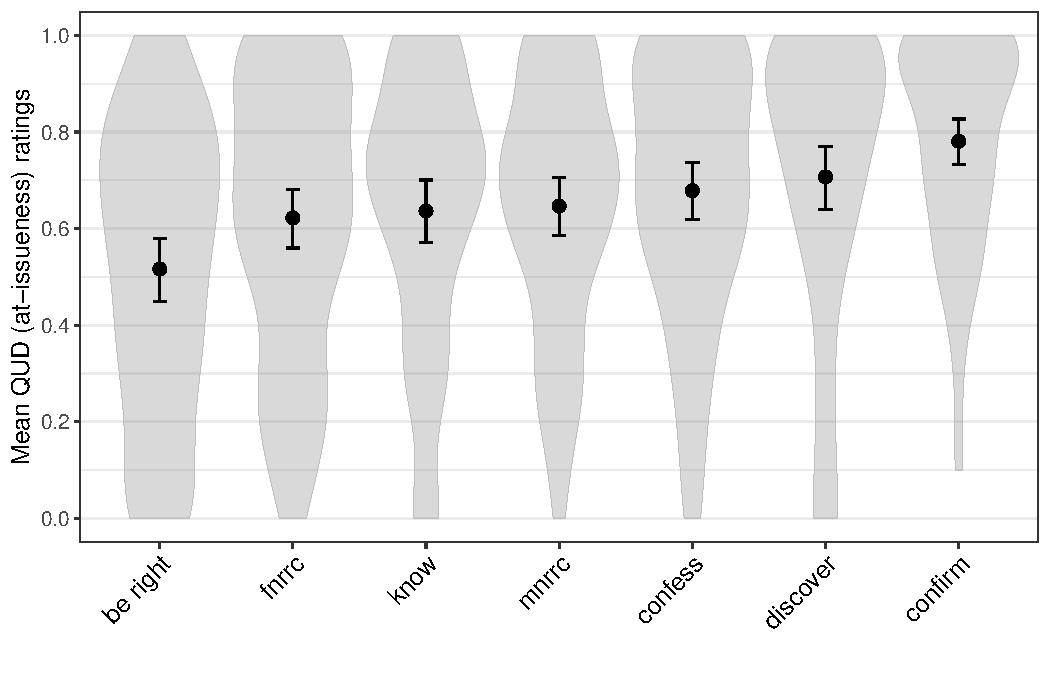
\includegraphics[width=.48\textwidth]{mean-QUD-ratings.pdf}
        \label{fig:qud}
    }
    \subfloat[`asking whether' ratings]{
        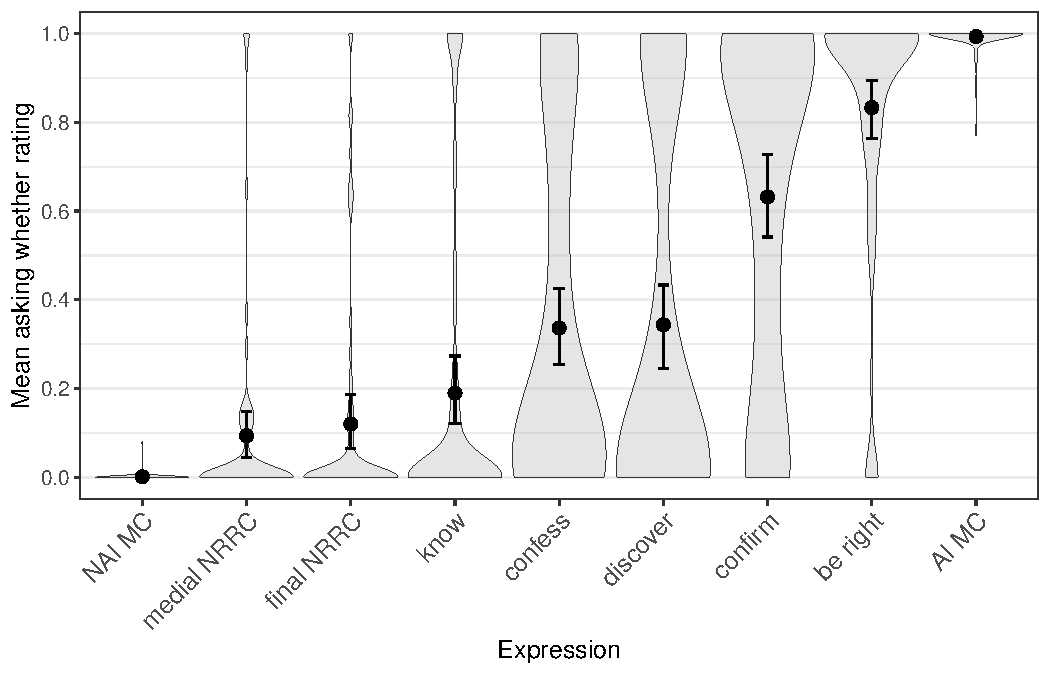
\includegraphics[width=.48\textwidth]{mean-AK-ratings.pdf}
        \label{fig:AK}
    }\\
    \vspace{-\baselineskip}
    \subfloat[Naturalness ratings for the `direct dissent' diagnostic]{
        \includegraphics[width=.48\textwidth]{mean-DD-ratings.pdf}
        \label{fig:dd}
    }

\end{figure}

\begin{figure}[htbp]
\vspace{-2\baselineskip}
  \caption{Proportion of ‘no’ choices by content for the `yes but' diagnostic. Error bars indicate 95\% bootstrapped confidence intervals. Gray dots indicate individual participant responses (either ‘no’ or one of the ‘yes’-responses, jittered vertically and horizontally for legibility).} \label{fig:yb}
  \vspace{-.5\baselineskip}
  \centering
  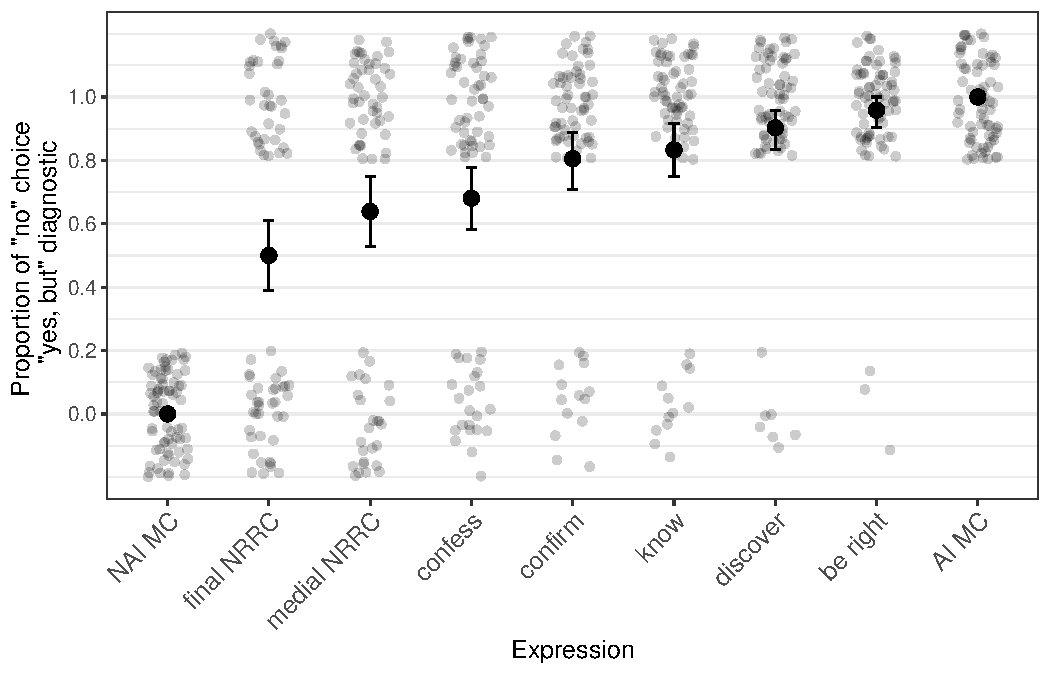
\includegraphics[width=.48\textwidth]{YB.pdf}
\end{figure}

\vspace{-.8\baselineskip}
\noindent \textbf{References.}
Yuqiu Chen. Presuppositions at the semantics-pragmatics interface. 2024.
 ~\textbullet~
%
Emilie Destruel, Edgar Onea, Daniel Velleman, Dylan Bumford, and David Beaver. A cross-linguistic study of the non-at-issueness of exhaustive inferences. In Floran Schwarz, editor, Experimental approaches to presupposition,
pages 135–156. Springer, 2015. ~\textbullet~
%
Katharina Drozdov. Projection and at-issueness of nonrestrictive relative clauses. Unpublished manuscript, 2024.
 ~\textbullet~
%
Todor Koev. Notions of at-issueness. Language and Linguistics Compass, 12(12):e12306, 2018.
 ~\textbullet~
%
Torgrim Solstad and Oliver Bott. Cataphoric resolution of projective content: The case of occasion verbs. Semantics and Pragmatics, 17(11):1–66, July 2024.
 ~\textbullet~
%
Kristen Syrett and Todor Koev. Experimental evidence for the truth conditional contribution and shifting information status of appositives. Journal of Semantics, 32(3):525–577, 2015.
 ~\textbullet~
%
Judith Tonhauser. Diagnosing (not-) at-issue content. Proceedings of Semantics of Under-represented Languages of the Americas (SULA), 6:239–254, 2012.
 ~\textbullet~
%
Judith Tonhauser, David I Beaver, and Judith Degen. How projective is projective content? gradience in projectivity and at-issueness. Journal of Semantics, 35(3):495–542, 2018.
 ~\textbullet~
%
Jingyang Xue and Edgar Onea. Correlation between presupposition projection and at-issueness: An empirical study.
In Proceedings of the ESSLLI 2011 workshop on projective meaning, pages 171–184, 2011.


\pagebreak
\bibliographystyle{plainnat}
\bibliography{mybib}

\end{document}